% !TeX spellcheck = en_GB
\documentclass[11pt]{article}

\usepackage[type1]{libertine}
\usepackage[a4paper]{geometry}
\usepackage{amsmath, amsthm, amssymb} 
\usepackage{parskip}
\usepackage{tabularx}
\usepackage[english]{babel}
\usepackage{enumitem}
\usepackage{gensymb}
\usepackage{bm}
\usepackage{graphicx}
\usepackage{xcolor}
\usepackage{float}
\usepackage{wrapfig}
\usepackage[makeroom]{cancel}
\usepackage{multicol}
\usepackage{commath} % Provides good differentials
\usepackage{siunitx} % Provides good units
\usepackage{nicefrac}

\usepackage[titletoc,title,toc,page]{appendix}
\usepackage{hyperref}
\hypersetup{
	pdftitle={Tutorial 3B (Dynamics) Worked Solutions},
	pdfauthor={Sun Yudong},
	bookmarksnumbered=true,
	bookmarksopen=true,
	bookmarksopenlevel=2,
	pdfstartview=Fit,
	pdfpagemode=UseOutlines,
	colorlinks=true,
	linkcolor=black,
	filecolor=magenta,      
	urlcolor=blue
}

\newcommand{\uvec}[1]{\boldsymbol{\hat{\textbf{#1}}}}
\newcommand{\solution}[1]{\textbf{Solution: } #1 \hspace{5mm}}

\newenvironment{multicolFigure}
{\par\medskip\noindent\minipage{\linewidth}}
{\endminipage\par\medskip}
% https://tex.stackexchange.com/questions/12262/multicol-and-figures

%\newenvironment{amatrix}[1]{%
%	\left(\begin{array}{@{}*{#1}{c} | c@{}}
%	}{%
%	\end{array}\right)
%}						% https://tex.stackexchange.com/a/2238
%\usepackage{blkarray}	% https://tex.stackexchange.com/a/59519
%\usepackage{mathtools}	% https://tex.stackexchange.com/a/103993

\title{Tutorial 3B (Dynamics) Worked Solutions}
\author{Sun Yudong\\Hwa Chong Institution}

\begin{document}
	\maketitle
	The following only contains the worked solutions to discussion questions in part 2 of Tutorial 3 (Conservation of Linear Momentum/Collisions). I have included some \hyperref[appdx]{appendices} to supplement the textbook.
	
	For Self-Review questions, please refer to the other uploaded document. 
	
	\begin{enumerate}
		\item[{[D12]}] \solution{A}
		
		Since the trolleys stick together on impact, $\vec{v_x} = \vec{v_y}$. The momentum of the entire system $\vec{p} = 0$ since it was stationary before the trolleys were released. Hence the final speed of Trolley Y $v_y = \nicefrac{p}{(M + 2M)} = 0$.
		
		Note that the force of the elastic band on the trolleys is an internal force and hence cannot change the momentum of the entire system.
		\vfill 
		\item[{[D13]}] \solution{C}
		
		Total momentum before the collision $= 6 \times 5.0 + 10 \times (-3.0) = 0$
		
		Each trolleys is decelerated to rest. Average force on each trolley = $\displaystyle \frac{\Delta P}{\Delta t} = \frac{30}{0.20} = 150$.
		\vfill
		\item[{[D14]}] 
		\begin{enumerate}
			\item \solution{\SI{721.4}{\meter\per\second}}
			
			All the momentum of the \SI{1.8}{\kilogram} block and the embedded bullet comes from the momentum of the bullet after it passes through the first block:
			\begin{align*}
				v_{bullet} &= \frac{p}{m_{bullet}} \\
				&= \frac{\left(1.8+3.5\times 10^{-3}\right)\times 1.4}{3.5\times 10^{-3}}\\
				&= \SI{721.4}{\meter\per\second}
			\end{align*}
			\pagebreak
			\item \solution{\SI{937.4}{\meter\per\second}}
			All the momentum of the \SI{1.8}{\kilogram} block, the embedded bullet and the \SI{1.2}{\kilogram} block comes from the original momentum of the bullet:
			\begin{align*}
			u_{bullet} &= \frac{p_{total}}{m_{bullet}} \\
			&= \frac{\left(1.8+3.5\times 10^{-3}\right)(1.4) + 1.2 (0.63)}{3.5\times 10^{-3}}\\
			&= \SI{937.4}{\meter\per\second}
			\end{align*}
		\end{enumerate}
		\item[{[D15]}] 
		\begin{enumerate}
			\item 
			\begin{enumerate}
				\item The linear momentum of a body is the product of its mass and its velocity. Mathematically, linear momentum, $\vec{p} = m\vec{v}$.
				\item The total linear momentum of a system is conserved if no net external force acts on the system. Mathematically:
				\begin{equation}
					\sum_{i} m_{i}u_{i} = \sum_{i} m_{i}v_{i} 
				\end{equation}
			\end{enumerate}
			\item 
			\begin{enumerate}
				\item Their relative speed of approach is equal to the relative speed of separation. Mathematically:
				\begin{equation}
					u_1 - u_2 = v_2 - v_1
				\end{equation}
				\item The direction of motion before and after the collision are along the same line of motion. 
			\end{enumerate}
			\item We define right as positive. 
			\begin{enumerate}
				\item \solution{\SI{2285}{\meter\per\second}} Since the collision is elastic, the relative speed of approach is equal to the relative speed of separation:
				\begin{align*}
					v_{sep} &= u_H - u_O \\
					&= 1.88\times 10^3 - (-405) = \SI{2285}{\meter\per\second}
				\end{align*}
				\item $m_Hu_H + m_Ou_O = m_Hv_H + m_Ov_O$
				\item \textcolor{white}{.}
				\vspace{-0.7cm}
				\begin{align}
					v_O - v_H &= 2285 \notag\\
					v_O = 2285 + v_H \label{eqn:D15:sep}
				\end{align}
				Substitute \eqref{eqn:D15:sep} into the equation in (c)ii:
				\begin{align*}
					m_Hv_H+m_O(2285 + v_H) &= (2.00)\left(1.88\times 10^3\right) + (32.0)(-405)\\
					v_H (m_H+m_O) &=-9200 - (2285)(32.0) \\
					v_H &= \frac{-82320}{2.00+32.0} = \underline{\SI{-2.42e3}{\meter\per\second}} \\
					v_O &= 2285 + v_H = \underline{\SI{-136}{\meter\per\second}}
				\end{align*}
			\end{enumerate}
		\end{enumerate}
		\pagebreak
		\item[{[D16]}]
		\begin{enumerate}
			\item The total momentum of the 2 nuclei is non-zero $\left(\sum p = 3mv - 2mv = mv\right)$
			\item \textcolor{white}{.}
			\vspace{-0.7cm}
			\begin{align*}
				p &= 5mv_s \\
				v_s &= \frac{\cancel{m}v}{5\cancel{m}} = \nicefrac{1}{5} v
			\end{align*}
			\item 
			\begin{enumerate}
				\item \textcolor{white}{.}
				\begin{figure}[ht!]
					\vspace{-0.7cm}
					\centering
					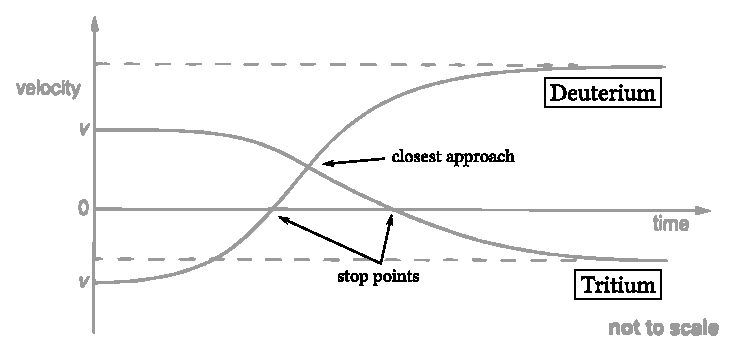
\includegraphics[width=10cm]{D16.eps}
				\end{figure}
				\item We define right as positive.
				\vspace{-0.2cm}
				\begin{align}
					p = (3\cancel{m})v_t + (2\cancel{m})v_d &= \cancel{m}v \notag\\
					2v_d + 3v_t &= v \label{eqn:d16:1}\\
					\left(u_t - u_d\right) = \left[v -(-v)\right] = 2v &= v_d - v_t \notag\\
					v_d - v_t &= 2v \label{eqn:d16:2}
				\end{align}
				$\eqref{eqn:d16:1} - 2\times\eqref{eqn:d16:2}:$
				\begin{align*}
					v_t &= -\nicefrac{3}{5}v = -0.6v\\
					v_d &= \left[2 + \left(-\nicefrac{3}{5}\right)\right]v = 1.4v
				\end{align*}
			\end{enumerate}
		\end{enumerate}
		\item[{[D17]}]
		\begin{enumerate}
			\item By the law of conservation of linear momentum, the total momentum of the system must be conserved. Since, by exhausting the gas, the gas from the rocket-gas system gains momentum, the toy car must gain momentum in the opposite direction in order to conserve total momentum. 
			
			Since $F = \od{p}{t}$, and there is a change in momentum, the rocket produces a forward force on the car. 
			\item 
			\begin{enumerate}
				\item 
				\begin{enumerate}[label={[\arabic*]}]
					\item $\displaystyle a = \text{grad} = \frac{16.0 - 2.8}{4.90-0.00} = \SI{2.7}{\meter\per\second\squared}$
					\item \textcolor{white}{.}
					\vspace{-0.5cm}
					\begin{align*}
						\sum F = ma &= F_{rocket} - F_r \\
						F_r &= F_{rocket} - ma \\
						&= 4.6 - \left(440\times 10^{-3}\right)(2.7) \\
						&= \SI{3.4}{\newton}
					\end{align*}
				\end{enumerate}
			\end{enumerate}
			\item The acceleration of the toy car at $t = 0$ is approximately $a = \SI{8.4}{\meter\per\second\squared}$, which is less than $g = \SI{9.81}{\meter\per\second\squared}$. Thus, it can be deduced that the rocket engine will not be able to produce a force large enough for the toy car to overcome the forces of gravity and travel vertically upwards. Thus, this suggestion is not very feasible. 
		\end{enumerate}
	\end{enumerate}
	
	\pagebreak
	\begin{appendices}
		\label{appdx}
		\section{Solving Collision Problems}
		\begin{enumerate}[label={\underline{Step \arabic*}}]
			\setcounter{enumi}{-1}
			\item Illustrate if no diagram is provided.
			\item Set up the PCOM equation, choosing an appropriate positive direction. \textbf{IF} collision is \textbf{perfectly inelastic}, use one variable to represent the final velocities of both bodies (i.e. let $v_1=v_2=v$)
			\item \textbf{IF} collision is elastic, set up the Relative Speed of Approach/Separation equation. If you aren't very sure, apply Conservation of Kinetic Energy.
			\item Solve for the unknowns, e.g. mass, initial or final velocities.
			
			You need as many independent equations as there are unknowns to solve them uniquely\footnote{If you are curious, for systems of linear equations, google linear independence, general solution to linear systems.}.
		\end{enumerate}
		\vfill
		\section{Coefficient of Restitution}
		The elasticity of a collision is quantified by a number called coefficient of restitution, $\varepsilon$, defined as the ratio of the speed of separation to the speed of approach:
		\begin{equation}
			\varepsilon = \frac{|\vec{v_2} - \vec{v_1}|}{|\vec{u_2} - \vec{u_1}|}
		\end{equation}
		A perfectly elastic collision has a coefficient of restitution $\varepsilon = 1$ (e.g. two diamonds bouncing off each other). 
		
		A perfectly plastic, or inelastic, collision has $\varepsilon = 0$ (e.g. two lumps of clay that don't bounce at all, but stick together.).
		
		So the coefficient of restitution will always be between zero and one. 
		
		$\varepsilon$ is determined by several factors, like the material of the colliding bodies, and \textit{assumed} to be independent of speed. 
		\vfill
		\pagebreak
		\section{Newton's Law in Car Safety}
		Using Newton's laws, discuss how each of the following features in vehicles increases the safety of its passengers:
		\begin{enumerate}
			\item Seat Belts
			\subitem Seat belt exerts a retardation force on the passenger, without which he would have continued in his state of uniform in a straight line into the windscreen (N1L).
			\subitem The vehicle is able to decelerate rapidly because of the braking system leads to a frictional force between the road surface and the tyres. Unfortunately, this frictional force acts on the vehicle, not the passenger. Without the seat belt, the only retardation force would be the frictional force between the seat and the passenger's bum. But this force is limited (recall: $f \leq \mu_s N$). If the vehicle decelerates too fast, the frictional force is not large enough to decelerate the passenger at the same rate as the vehicle.
			\subitem Be very clear that when passengers crash into the windscreen, it was due to their inertia. It was not due to some mysterious ``forward force".
			\item Head Restraints
			\subitem If the car is hit from the rear, the restraints provides a forward force on the passenger's head so that the head is accelerated at the same rate as the rest of his body, so that he does not suffer from whiplash (neck injury). 
			\item Air Bags
			\subitem Air bags exerts a relatively small force over a relatively long duration of time, safely bringing the passenger to rest by reducing the passenger's momentum at a relatively slower rate (N2L).
		\end{enumerate}
	\end{appendices}
\end{document}